% ######################################################################################################################
%         Supporting Information
% ######################################################################################################################

\chapter{Supporting Information}
\label{ch:SupportingInformation}

\begin{table}[htbp]
\caption[IUPAC notation of nucleobases and ambiguity characters]{
\textbf{IUPAC notation of nucleobases and ambiguity characters.}
The table lists the character representations of nucleobases and their combinations (which are used to denote ambiguity)
as suggested by the IUPAC (International Union of Pure and Applied Chemistry) Commission \cite{IUPAC1970}.
The names and symbols for ambiguity characters are chosen based on bio-chemical properties of the nucleobases.
See \secref{ch:Foundations:sec:SequenceAnalysis:sub:ConsensusSequences} for more information.
}
\label{tab:AmbiguityCharacters}
{
    \newcommand{\mc}[3]{\multicolumn{#1}{#2}{#3}}
    \newcommand{\rb}{\cellcolor{black!12}}
    \begin{center}
    \begin{tabular}{c|l|cccc|c|c}
%     \toprule
    \hline
    Symbol & Description & \mc{5}{c|}{Represented Bases} & Complement \\
%     \midrule
    \hline
    A & \textbf{A}denine & \rb{} A &  &  &  & 1 & T \\
    C & \textbf{C}ytosine &  & \rb{} C &  &  & 1 & G \\
    G & \textbf{G}uanine &  &  & \rb{} G &  & 1 & C \\
    T & \textbf{T}hymine &  &  &  & \rb{} T & 1 & A \\
    U & \textbf{U}racil &  &  &  & \rb{} U & 1 & A \\
    \hline
    W & \textbf{W}eak & \rb{} A &  &  & \rb{} T & 2 & W \\
    S & \textbf{S}trong &  & \rb{} C & \rb{} G &  & 2 & S \\
    M & a\textbf{M}ino & \rb{} A & \rb{} C &  &  & 2 & K \\
    K & \textbf{K}eto &  &  & \rb{} G & \rb{} T & 2 & M \\
    R & pu\textbf{R}ine & \rb{} A &  & \rb{} G &  & 2 & Y \\
    Y & p\textbf{Y}rimidine &  & \rb{} C &  & \rb{} T & 2 & R \\
    \hline
    B & not A (\textbf{B} comes after A) &  & \rb{} C & \rb{} G & \rb{} T & 3 & V \\
    D & not C (\textbf{D} comes after C) & \rb{} A &  & \rb{} G & \rb{} T & 3 & H \\
    H & not G (\textbf{H} comes after G) & \rb{} A & \rb{} C &  & \rb{} T & 3 & D \\
    V & not T (\textbf{V} comes after T and U) & \rb{} A & \rb{} C & \rb{} G &  & 3 & B \\
    \hline
    N & any \textbf{N}ucleotide (not a gap) & \rb{} A & \rb{} C & \rb{} G & \rb{} T & 4 & N \\
    Z & \textbf{Z}ero &  &  &  &  & 0 & \\
%     \bottomrule
%     \hline
    \end{tabular}
    \end{center}
}
\end{table}

\begin{figure}[thb!p]
    \centering
    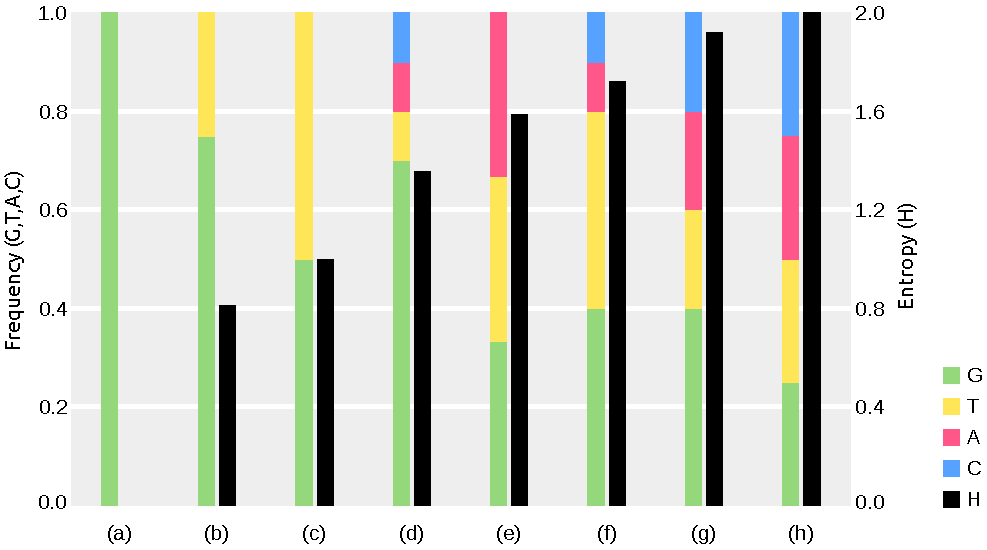
\includegraphics[width=\linewidth]{entropy.pdf}
    \begin{subfigure}{0pt}
        \phantomcaption
        \label{fig:entropy:sub:a}
    \end{subfigure}
    \begin{subfigure}{0pt}
        \phantomcaption
        \label{fig:entropy:sub:b}
    \end{subfigure}
    \begin{subfigure}{0pt}
        \phantomcaption
        \label{fig:entropy:sub:c}
    \end{subfigure}
    \begin{subfigure}{0pt}
        \phantomcaption
        \label{fig:entropy:sub:d}
    \end{subfigure}
    \begin{subfigure}{0pt}
        \phantomcaption
        \label{fig:entropy:sub:e}
    \end{subfigure}
    \begin{subfigure}{0pt}
        \phantomcaption
        \label{fig:entropy:sub:f}
    \end{subfigure}
    \begin{subfigure}{0pt}
        \phantomcaption
        \label{fig:entropy:sub:g}
    \end{subfigure}
    \begin{subfigure}{0pt}
        \phantomcaption
        \label{fig:entropy:sub:h}
    \end{subfigure}
    \caption[Examples of the per-site entropy for different character frequencies]{
        \textbf{Examples of the per-site entropy for different character frequencies.}
        The figure shows the entropy $H$ that results from an alignment site with some exemplary nucleotide frequencies.
        See \secref{ch:AutomaticTrees:sec:Methods:sub:PhAT:par:SequenceEntropy}
        for details of the calculation of the per-site entropy,
        and for its application in the context of multiple sequence alignments.
        The entropy is symmetric with respect to permutations of the nucleobases;
        we here show examples using the nucleobase \nucleobase{G} as the most frequent character at the site.
        For simplicity, we here do not include the gap character.
        \\
        The subfigures are ordered by increasing entropy,
        which ranges from $0$ for a site with only a single character, as in \subref{fig:entropy:sub:a},
        to $2$ for a site with all four nucleobases equally frequent, as in \subref{fig:entropy:sub:h}.
%         \subref{fig:entropy:sub:a} The site only contains one character, the resulting entropy is $0$.
%         \subref{fig:entropy:sub:b}, \subref{fig:entropy:sub:c} Another character appears with 25\% and 50\% frequency, respectively.
%         \subref{fig:entropy:sub:d} One character appears with 70\% frequency, the three remaining ones with 10\% each.
%         \subref{fig:entropy:sub:e} Three characters with equal frequency of 33.3\% each.
%         \subref{fig:entropy:sub:f} Two characters with 40\%, and two with 10\% frequency.
%         \subref{fig:entropy:sub:g} One character with 40\%, and three with 20\% frequency each.
%         \subref{fig:entropy:sub:h} All four characters are equally frequent with 25\% each, resulting in the maximum entropy of $2$.
        The maximum possible entropy is given by the base of the logarithm.
        The choice of base is irrelevant when comparing entropies with each other,
        as it simply introduces a constant factor.
    }
    \label{fig:entropy}
\end{figure}
